Per prima cosa si procede all'assemblaggio dell'apparato sperimentale, come mostra la Figura (3). Successivamente è stato fissato al muro lo schermo in Figura (4) in modo tale che su di esso potesse essere possibile visualizzare l'angolo di minima deviazione. A questo punto è stato misurato l'intervallo di minima deviazione, ovvero il range di valori dell'angolo di incidenza $\theta_i$ per cui l'angolo di deviazione $\delta$ del raggio emergente si mantiene pressoché costante. All'interno di questo intervallo, piccole variazioni dell'angolo di incidenza non producono variazioni apprezzabili nell'angolo di deviazione.

\begin{equation}
	\theta_{i_{min}}\in[35,\ 37]^\circ
\end{equation}
Ovvero
\begin{equation}
	\theta_{i_{min}}=(36\pm 1)^\circ
\end{equation}

Terminata l'individuazione dell'intervallo di minima deviazione, si è proceduto alla misura degli angoli di incidenza $(\theta_i)$, incrementandoli progressivamente e segnandone il punto di intersezione del raggio laser sullo schermo, fino a raggiungere il valore corrispondente alla minima deviazione. Superato il minimo si sono registrati gli angoli di incidenza $(\theta_i')$, via via maggiori, corrispondenti ad ogni punto segnato sullo schermo precedentemente. In questo modo, dalla Legge (1) e considerando $\alpha=45^\circ$, è stato possibile stimare gli angoli di deviazione.

\begin{table}[H]
	\centering
	\begin{tabular}{|c|c|c|}
		\hline
		$\theta_i \ (^\circ)$ & $\theta_i' \ (^\circ)$ & $\delta \ (^\circ)$ \\
		\hline
		$9.0\pm 0.5$ & $69.0\pm 0.5$ & $33.0\pm 1.0$ \\
		\hline
		$10.0\pm 0.5$ & $66.5\pm 0.5$ & $31.5\pm 1.0$ \\
		\hline
		$11.0\pm 0.5$ & $64.5\pm 0.5$ & $30.5\pm 1.0$ \\
		\hline
		$12.0\pm 0.5$ & $62.5\pm 0.5$ & $29.5\pm 1.0$ \\
		\hline
		$13.0\pm 0.5$ & $61.0\pm 0.5$ & $29.0\pm 1.0$ \\
		\hline
		$14.0\pm 0.5$ & $59.5\pm 0.5$ & $28.5\pm 1.0$ \\
		\hline
		$15.0\pm 0.5$ & $58.0\pm 0.5$ & $28.0\pm 1.0$ \\
		\hline
		$16.0\pm 0.5$ & $56.5\pm 0.5$ & $27.5\pm 1.0$ \\
		\hline
		$17.0\pm 0.5$ & $55.0\pm 0.5$ & $27.0\pm 1.0$ \\
		\hline
		$18.0\pm 0.5$ & $53.5\pm 0.5$ & $26.5\pm 1.0$ \\
		\hline
		$19.0\pm 0.5$ & $52.5\pm 0.5$ & $26.5\pm 1.0$ \\
		\hline
		$20.0\pm 0.5$ & $50.5\pm 0.5$ & $25.5\pm 1.0$ \\
		\hline
		$21.0\pm 0.5$ & $49.5\pm 0.5$ & $25.5\pm 1.0$ \\
		\hline
		$22.0\pm 0.5$ & $48.5\pm 0.5$ & $25.5\pm 1.0$ \\
		\hline
		$23.0\pm 0.5$ & $47.5\pm 0.5$ & $25.5\pm 1.0$ \\
		\hline
		$24.0\pm 0.5$ & $45.5\pm 0.5$ & $24.5\pm 1.0$ \\
		\hline
		$25.0\pm 0.5$ & $45.0\pm 0.5$ & $25.0\pm 1.0$ \\
		\hline
		$28.0\pm 0.5$ & $41.5\pm 0.5$ & $24.5\pm 1.0$ \\
		\hline
	\end{tabular}
	\captionsetup{width=0.7\linewidth}
	\caption{Le misurazioni degli angoli $\theta_i$ e $\theta_i'$ sono state effettuate utilizzando la piattaforma rotante graduata. L'incertezza associata a queste due grandezze è quella strumentale. L'incertezza valutata su $\delta$ è ottenuta tenendo conto della propagazione dell'errore (vedi Sezione (2.3)).}
	\label{tab:}
\end{table}

I dati sperimentali in Tabella (2) sono stati poi rappresentati in un grafico.

\begin{figure}[H]
	\centering
	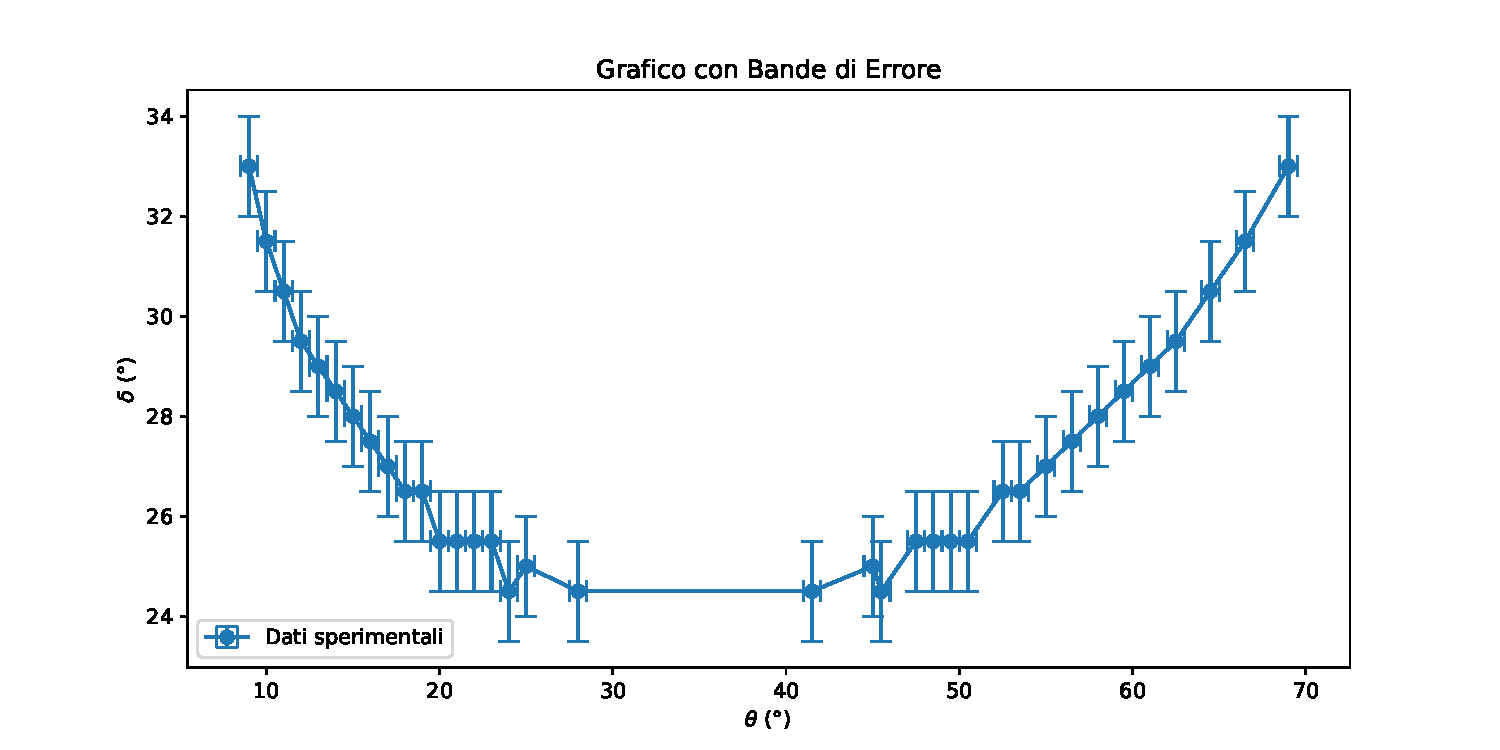
\includegraphics[width=0.95\textwidth]{./figures/grafico1.pdf}
	\captionsetup{width=0.7\linewidth}
	\caption{Sull'asse delle ascisse sono presenti i valori relativi agli angoli di incidenza misurati sperimentalmente. Sull'asse delle ordinate sono invece riportati i rispettivi angoli di deviazione per ognuno degli angoli di incidenza.}
\end{figure}

Dalla Legge (2) e tenendo conto della (22) e del valore di $\alpha=45^{\circ}$ è possibile calcolare l'indice di rifrazione del prisma. L'incertezza è stata valutata tenendo conto della propagazione dell'errore (vedi Sezione (2.3)).

\begin{equation}
	\Delta n=\left(\frac{\cos(\theta_{i_{min}})}{\sin(\frac{\alpha}{2})}\right)\Delta \theta_{i_{min}}=0.04^{\circ}
\end{equation}
E quindi
\begin{equation}
	n = (1.54\pm 0.04)^{\circ}
\end{equation}